% This file was created by matlab2tikz.
%
%The latest updates can be retrieved from
%  http://www.mathworks.com/matlabcentral/fileexchange/22022-matlab2tikz-matlab2tikz
%where you can also make suggestions and rate matlab2tikz.
%
\definecolor{mycolor1}{rgb}{0.00000,0.44700,0.74100}%
\definecolor{mycolor2}{rgb}{0.85000,0.32500,0.09800}%
%
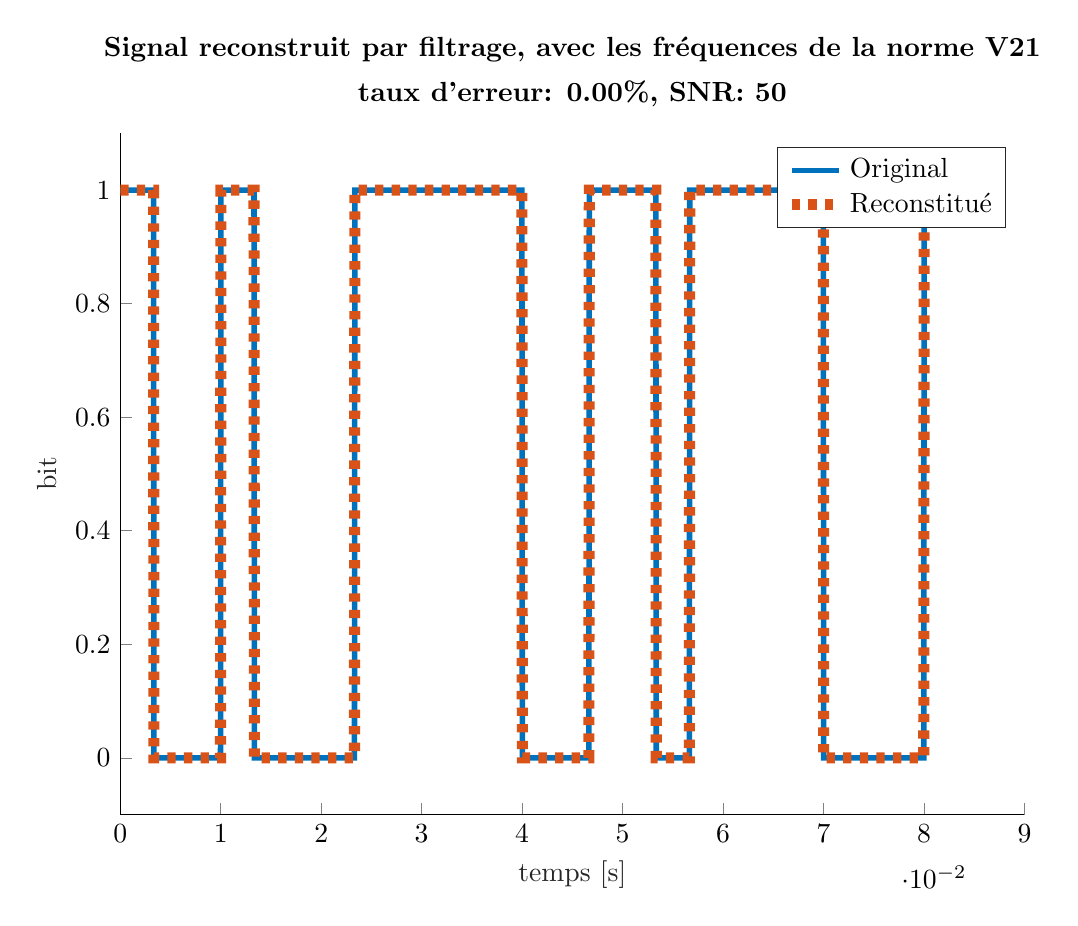
\begin{tikzpicture}

\begin{axis}[%
width=4.521in,
height=3.406in,
at={(0.758in,0.488in)},
scale only axis,
xmin=0,
xmax=0.09,
xlabel style={font=\color{white!15!black}},
xlabel={temps [s]},
ymin=-0.1,
ymax=1.1,
ylabel style={font=\color{white!15!black}},
ylabel={bit},
axis background/.style={fill=white},
title style={font=\bfseries, align=center},
title={Signal reconstruit par filtrage, avec les fréquences de la norme V21\\[1ex]taux d'erreur: 0.00\%, SNR: 50},
axis x line*=bottom,
axis y line*=left,
legend style={legend cell align=left, align=left, draw=white!15!black}
]
\addplot [color=mycolor1, line width=2.0pt]
  table[row sep=crcr]{%
0	1\\
0.00331250000000005	1\\
0.00335416666666677	0\\
0.00997916666666665	0\\
0.0100208333333334	1\\
0.0133125000000001	1\\
0.0133541666666668	0\\
0.0233125000000001	0\\
0.0233541666666666	1\\
0.0399791666666667	1\\
0.0400208333333334	0\\
0.0466458333333333	0\\
0.0466875	1\\
0.0533125000000001	1\\
0.0533541666666666	0\\
0.0566458333333333	0\\
0.0566875	1\\
0.0699791666666667	1\\
0.0700208333333334	0\\
0.0799791666666667	0\\
0.0800208333333334	1\\
0.0833124999999999	1\\
};
\addlegendentry{Original}

\addplot [color=mycolor2, dashed, line width=4.0pt]
  table[row sep=crcr]{%
0	1\\
0.00331250000000005	1\\
0.00335416666666677	0\\
0.00997916666666665	0\\
0.0100208333333334	1\\
0.0133125000000001	1\\
0.0133541666666668	0\\
0.0233125000000001	0\\
0.0233541666666666	1\\
0.0399791666666667	1\\
0.0400208333333334	0\\
0.0466458333333333	0\\
0.0466875	1\\
0.0533125000000001	1\\
0.0533541666666666	0\\
0.0566458333333333	0\\
0.0566875	1\\
0.0699791666666667	1\\
0.0700208333333334	0\\
0.0799791666666667	0\\
0.0800208333333334	1\\
0.0833124999999999	1\\
};
\addlegendentry{Reconstitué}

\end{axis}
\end{tikzpicture}%